\section{Hauptarchitektur des CNN}
%
Die Netzarchitektur, die sich im Laufe dieser Arbeit als die Effektivste
herausgestellt hat (i.F. Hauptarchitektur), ist in Tabelle~\ref{tab:haupt} dargestellt. Es hat
sich im Laufe der Bearbeitung zunächst herausgestellt, dass die Kombination
aus \texttt{Conv2D} Lage und \texttt{MaxPooling} Lage eine gut
funktionierende Grundlage für das vorliegende Problem ist.
Daher besitzt die Hauptarchitektur zwei Einheiten dieser Kombination
direkt zu Beginn des Netzes. Hier soll also die Zerlegung der Bilder auf
die in Abschnitt~\ref{sec:netze} beschriebene Weise stattfinden.
Die beiden \texttt{Conv2D} Lagen rastern das Bild über einen $4\times4$
Kernel ab. Daher entstehen die in Tabelle~\ref{tab:haupt} aufgeführten
Dimensionen. Das Bild wird mit $(2, 2)$ \textit{strides} durchfahren,
sodass sich die Dimension des Bildes von $400\times400$ zunächst auf
$199\times199$ reduziert. Eine \texttt{MaxPooling} Lage reduziert diese
mit $(3, 3)$ \textit{strides} auf $66\times66$. Die folgende Einheit
aus  \texttt{Conv2D} und \texttt{MaxPooling} Lage lieferen schließlich
einen Output der Dimension $10\times10$.\\
Dieser Output wird schließlich in den vollständig vernetzten Teil des
Netzes gespeist. Hierbei hat sich gezeigt, dass sowohl eine kleine Anzahl
Filter in der Größenordnung $64$ als auch eine sehr große Zahl der
Größenordnung $1000$ die Leistung des Netzes verringern. Bei einer sehr großen
Anzahl an Filtern in den Dichtelagen liegt der überwiegende Teil der
trainierbaren Parameter in einer Dichtelage. Diese Übergewichtung einer Lage
wird mit kleineren Dichtelagen verhindert. Außerdem reduziert sich so die
Gesamtgröße des Netzes, was sich signifikant in der Rechenzeit niederschlägt.
Daher sind hier fünf Dichtelagen mit den angegeben Größen implementiert.
Die Anzahl der Dichtelagen wurde dabei lediglich händisch variiert und das
beste Ergebnis gewählt.
%
\begin{table}[htb]
  \centering%
  \begin{tabular}{l
                  l
                  l}
      \toprule
      Layer (type)    & Output Shape     & Anzahl Parameter      \\
      \midrule
      Conv 2D         & (199, 199, 64)  & 1\,088 \\
      Max Pooling 2D  & (66, 66, 64)    & 0 \\
      Conv 2D         & (32, 32, 32)    & 32\,800 \\
      Max Pooling 2D  & (10, 10, 32)    & 0 \\
      Dropout (0,25)  & (10, 10, 32)    & 0 \\
      Dense           & (10, 10, 256)   & 8\,448 \\
      Dense           & (10, 10, 128)   & 32\,896 \\
      Flatten         & (12\,800)         & 0 \\
      Dense           & (100)           & 1\,280\,100 \\
      Dropout (0,5)   & (100)           & 0 \\
      Dense           & (32)            & 3\,232 \\
      Dense           & (4)             & 132 \\
      \midrule
      Gesamtanzahl Parameter &                & 1\,358\,696 \\
      \bottomrule
  \end{tabular}
  \caption{Einzelne Lagen, sowie die jeweiligen Dimensionen des Outputs für für Hauptarchitektur des CNN.}
  \label{tab:haupt}
\end{table}
%
Eine automatisierte Suche nach der besten Architektur in Form einer
Optimierungsstudie ist für dieses Netz mit den dafür zur Verfügung stehenden
Mitteln in endlicher Zeit nicht umzusetzen. Der hohe Bedarf an Arbeitsspeicher
und CPU-Leistung steht leider nicht zur Verfügung. Allerdings zeigte sich durch
etwa ein Dutzend Iterationen, dass das hier vorliegende Netz gute Leistungen
erbringt. Zwischen dem CNN und dem vollständig vernetzten Netz sowie vor
den letzten beiden Dichtelagen wird außerdem \texttt{Dropout} angewandt.
Dabei werden einzelne Knoten innerhalb des Netzes mit einer spezifizierten Rate
vom Training exkludiert. Das Training erfolgt also auf einem zufällig
generierten Teilnetz. Dies stellt eine sehr einfache und kostengünstige Art
der Regularisierung dar.\\
Durch die \texttt{Dropout} Lagen wird verhindert, dass ein so großes Netz zu schnell übertrainiert wird. \\
Die nichtlinearen Aktivierungsfunktionen in dieser Architektur sind in allen
entsprechenden Lagen \textit{exponential linear unit} (\textbf{elu}) Funktionen und in der letzten Lage die
\textbf{softmax} Funktion. Diese gewährleistet die Interpretation des
Netz-Outputs als Wahrscheinlichkeit für eine bestimmte Klasse.
Die \textbf{elu} Funktionen zeigten für verschiedene Architekturen die beste
Leistung. Im Vergleich z.B. zur \textit{rectified linear unit} (\textbf{relu}) Funktion zeigte sich allerdings
lediglich ein leichter Vorteil der \textbf{elu} Funktion.\\
Das Modell wurde 40 Epochen lang mit einer \textit{batch size} von 100 Bildern
trainiert. Das bedeutet, dass immer 100 Bilder gleichzeitig durch das Netz
propagieren. Dies wird innerhalb einer Epoche wiederholt, bis alle Bilder
verwendet wurden. Als Metrik für die Quantifizierung der Verbesserung des
Netzes wurde die Genauigkeit verwendet und als Verlustfunktion die
kategorische Kreuzentropie. Der Optimierer, der sich hier als am besten zeigte
ist der Adam Optimierer.

\section{Training}
%
Das Netz wurde auf $\SI{70}{\percent}$ des Datensatzes, also insgesamt
$57\,598$ Bildern trainiert und auf \SI{30}{\percent} validiert. Dabei ist die
Verteilung der Bilder auf die einzelnen Klassen jedoch nicht homogen, wie in
Tabelle~\ref{tab:count} dargestellt.
%
\begin{table}[htb]
  \centering%
  \begin{tabular}{l
                  l
                  l
                  l}
      \toprule
      NORMAL    & CNV    & DME & DRUSEN \\
      \midrule
      26315     & 37205  & 11348 & 8616 \\
      \bottomrule
  \end{tabular}
  \caption{Verteilung der Bilder auf die einzelnen Klassen.}
  \label{tab:count}
\end{table}
%
Eine solch ungleiche Verteilung hat vermutlich zur Folge, dass das Netz sehr
stark darauf konditioniert wird die Klasse mit vielen Bildern zu erkennen und
dafür die kleineren Klassen zu vernachlässigen. Außerdem wird so die
Genauigkeit verzerrt, da auch der Validierungsdatensatz diese Verteilung
widerspiegelt. Um dieser Problematik zu begegnen werden dem Netz zum Training
auch noch Gewichte für die einzelnen Bilder übergeben. Diese sind einheitlich
für jede Klasse und gleichen genau diese Unterschiede aus.
In Abbildung~\ref{fig:eq_all} sind zum Vergleich die Verwirrungsmatrizen
für ein gewichtetes Training, sowie für ein ungewichtetes Training dargestellt.
Die \textit{performance plots} sind allesamt auf einem Validierungsdatensatz
von insgesamt $24\,686$ Bildern entstanden, welcher dieselbe Verteilung auf
die einzelnen Klassen aufweist, wie der Trainingsdatensatz.
%
\begin{figure}[h!]
  \subcaptionbox{\label{fig:g}}{\centering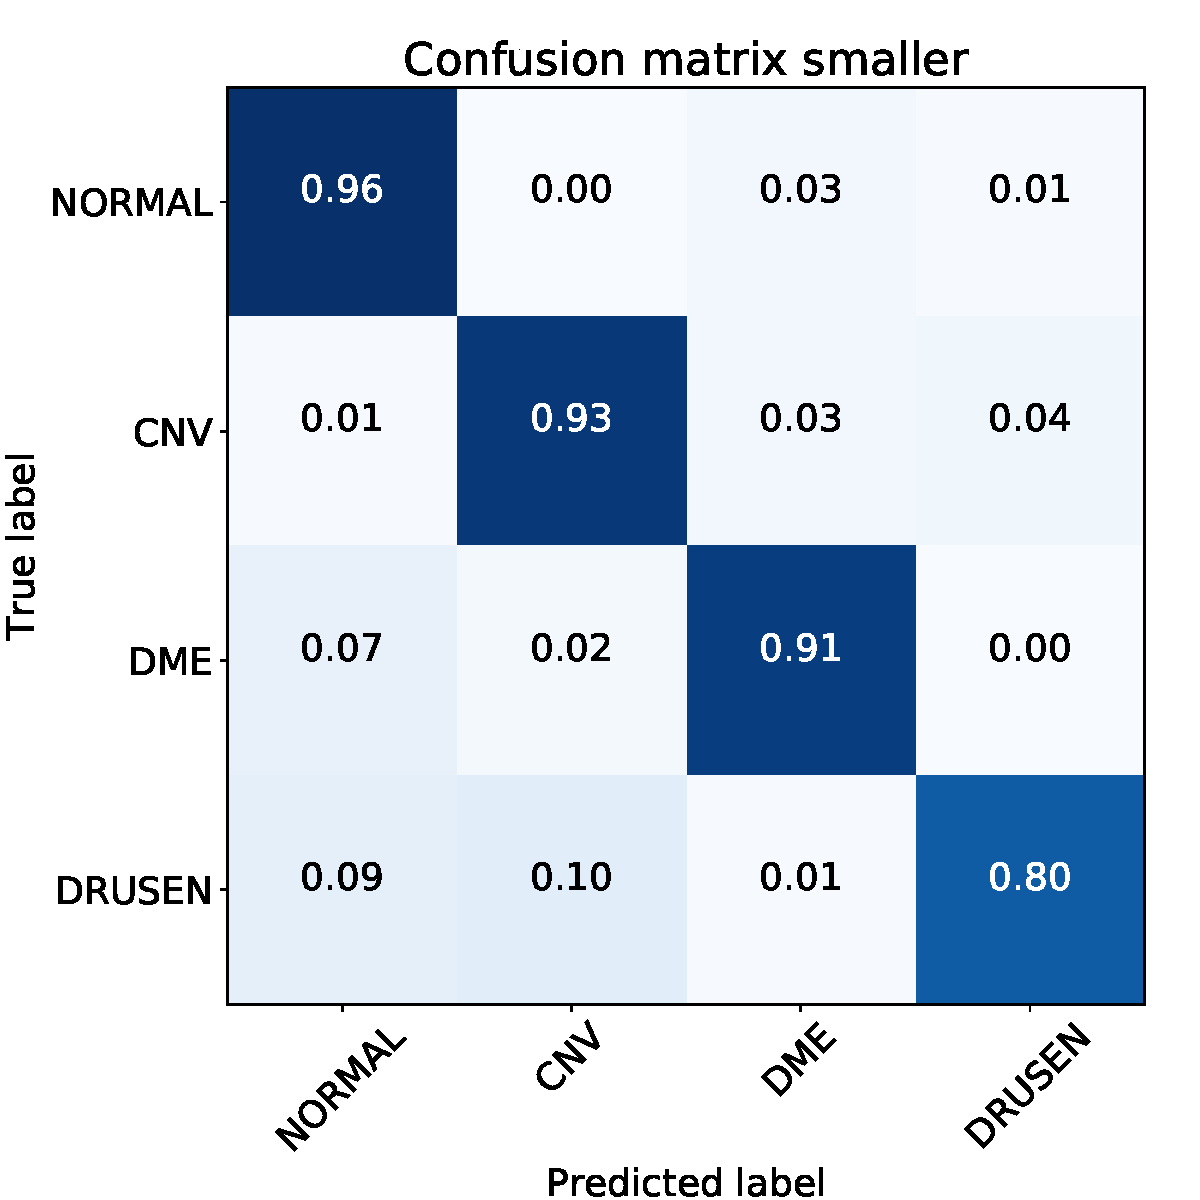
\includegraphics[width=0.4\textwidth]{Plots/confusion_matrix_smaller.pdf}}
  \hspace{8pt}
  \subcaptionbox{\label{fig:ug}}{\centering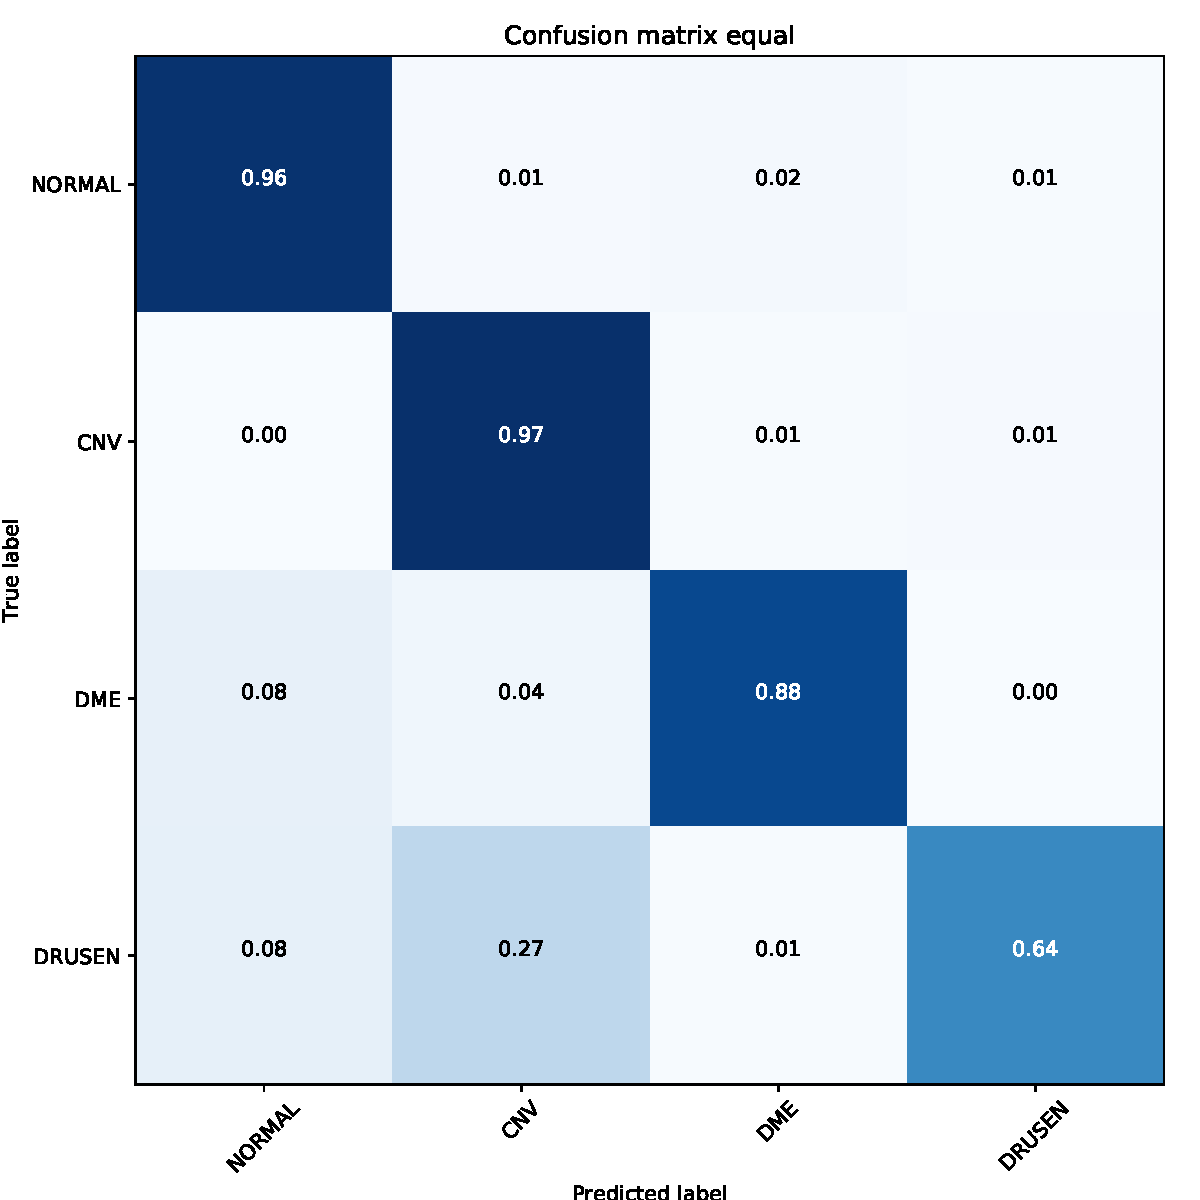
\includegraphics[width=0.4\textwidth]{Plots/confusion_matrix_equal.pdf}}
  \caption{Die Verwirrungsmatrix für das gewichtete \protect\subref{fig:g} und das ungewichtete Training \protect\subref{fig:ug}.}\label{fig:eq_all}
\end{figure}
%
Ein Netz, welches einwandfrei alle Klassen erkennen kann würde eine
Diagonalmatrix liefern. Allerdings zeugt auch eine diagonal-dominante Matrix
von einer gut funktionierenden Trennung. In diesem Falle sind die Einträge der
Matrix auf die Gesamtzahl der Bilder jeder wahren Klasse normiert, sodass die
Diagonaleinträge direkt die Genauigkeit für die explizite Klasse angeben.
Hierbei zeigt sich klar, dass bei dem ungewichteten Training wie erwartet die
Genauigkeiten für die Klassen mit vielen Bildern stark zunimmt, während die
kleinste Klasse (hier DRUSEN) am schlechtesten erkannt wird. Um dennoch von
einem möglichst großen Datensatz zu profitieren, wurde das Modell mit dem
gesamten Datensatz gewichtet trainiert.
%
\begin{figure}[h!]
  \subcaptionbox{DME}{\centering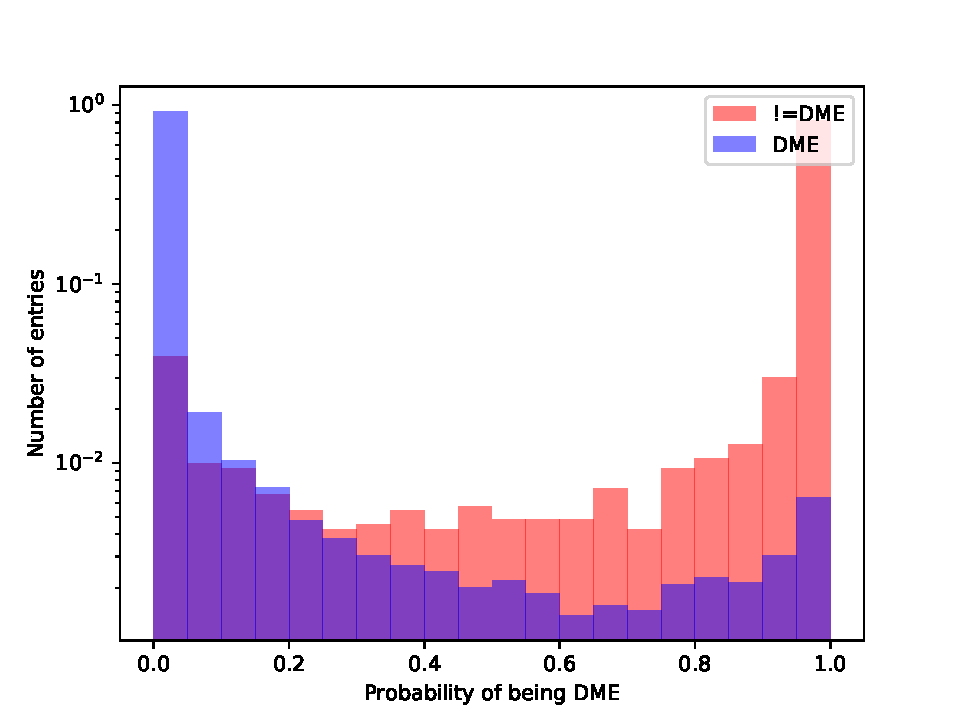
\includegraphics[width=0.48\linewidth]{Plots/DME_or_not_log_smaller.pdf}}
  \hspace{8pt}
  \subcaptionbox{CNV}{\centering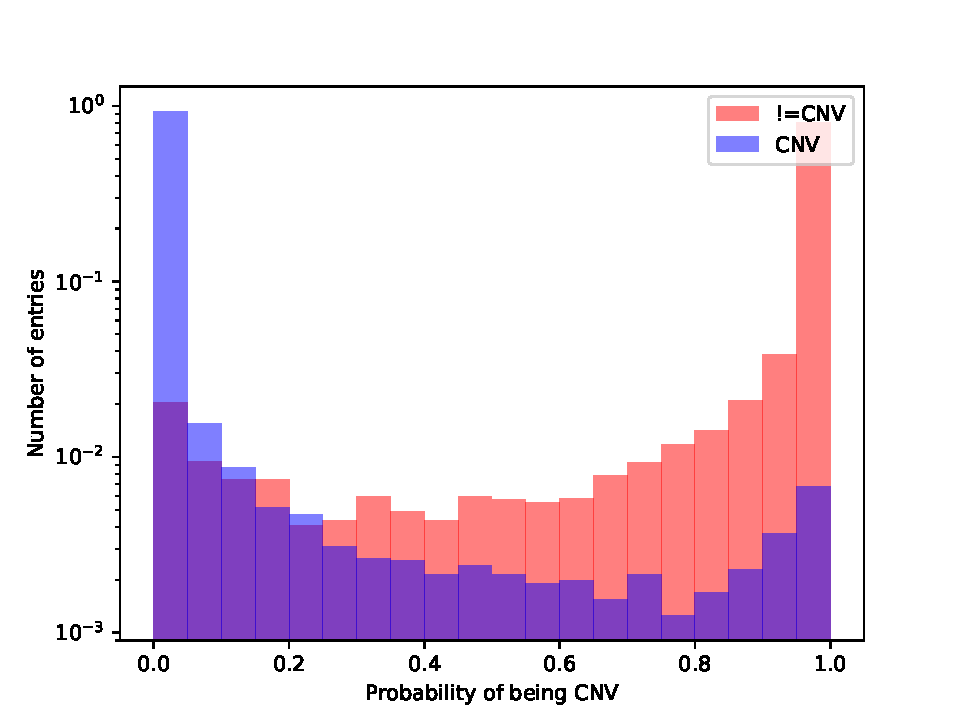
\includegraphics[width=0.48\linewidth]{Plots/CNV_or_not_log_smaller.pdf}}
  \subcaptionbox{DRUSEN}{\centering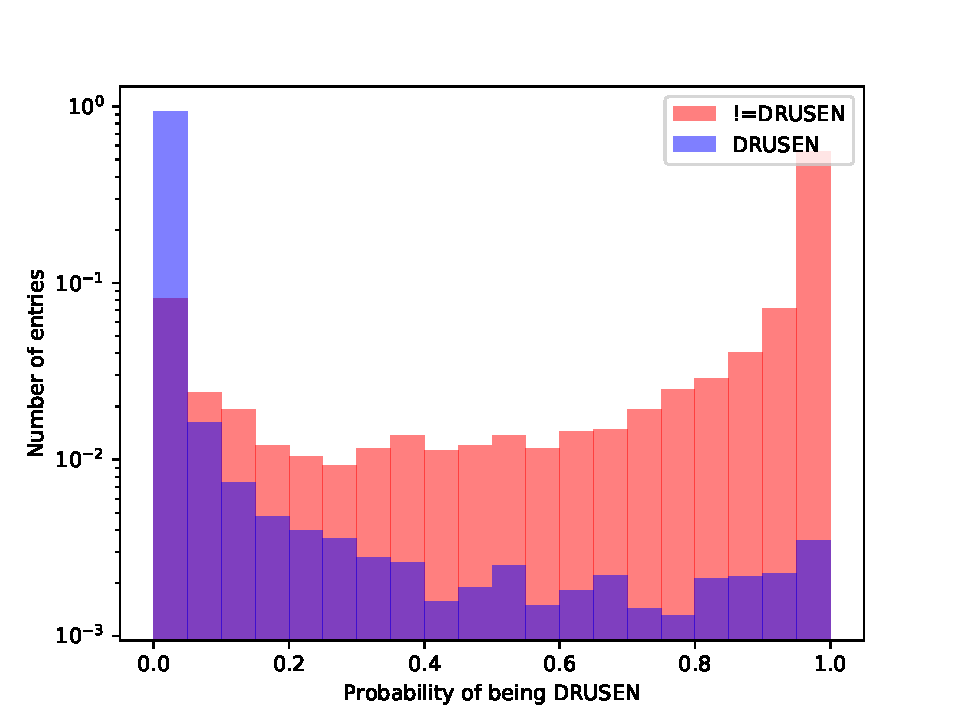
\includegraphics[width=0.48\linewidth]{Plots/DRUSEN_or_not_log_smaller.pdf}}
  \hspace{8pt}
  \subcaptionbox{NORMAL}{\centering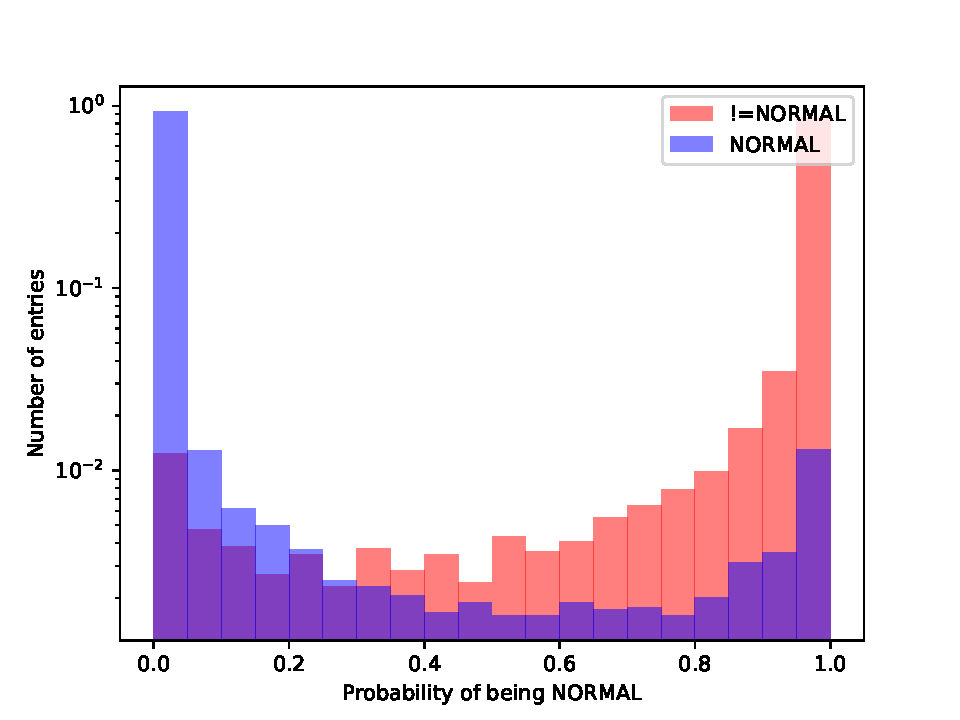
\includegraphics[width=0.48\linewidth]{Plots/NORMAL_or_not_log_smaller.pdf}}
  \caption{Ausgabe des Netzes für Bilder der einzelnen Klassen (normiert auf die Gesamtzahl der Klasse). Durch die softmax Funktion kann der Ausgabewert als Wahrscheinlichkeit für die Angehörigkeit zu einer Klasse interpretiert werden. Zwei Bins der Höhe 1 bei 0 und 1 würden eine perfekte Trennung repräsentieren.}
\end{figure}
%
